\documentclass[11pt,a4paper,twoside]{article}

% LaTeX-Umsetzung der "Richtlinien f�r Projekt- und Diplomarbeiten"
% der LFE Medieninformatik, LMU M�nchen. (Autor: Richard Atterer, 27.9.2006, 23.10.2007), Bug-Fixing Mark Kaczkowski (23.6.2008)

\usepackage[T1]{fontenc} % sonst geht \hyphenation nicht mit Umlauten
\usepackage[latin1]{inputenc} % man kann schreiben ����, statt "a"o"u"s
%\usepackage[utf8]{inputenc} % wie oben, aber UTF-8 als Encoding statt ISO-8859-1 (latin1)
\usepackage[ngerman,english]{babel} % deutsche Trennregeln, "Inhaltsverzeichnis" etc.
%\usepackage{ngerman} % Alternative zum Babel-Paket oben
%\usepackage{mathptmx} % Times-Roman-Schrift (auch f�r mathematische Formeln)


\usepackage{lmodern}

% Zum Setzen von URLs
\usepackage{color}
\definecolor{darkred}{rgb}{.25,0,0}
\definecolor{darkgreen}{rgb}{0,.2,0}
\definecolor{darkmagenta}{rgb}{.2,0,.2}
\definecolor{darkcyan}{rgb}{0,.15,.15}
\usepackage[plainpages=false,bookmarks=true,bookmarksopen=true,colorlinks=true,
  linkcolor=darkred,citecolor=darkgreen,filecolor=darkmagenta,
  menucolor=darkred,urlcolor=darkcyan]{hyperref}

% pdflatex: Bilder in den Formaten .jpeg, .png und .pdf
% latex: Bilder im .eps-Format
\usepackage{graphicx}

\usepackage{fancyhdr} % Positionierung der Seitenzahlen
\fancyhead[LE,RO,LO,RE]{}
\fancyfoot[CE,CO,RE,LO]{}
\fancyfoot[LE,RO]{\Roman{page}}
\renewcommand{\headrulewidth}{0pt}
\setlength{\headheight}{13.6pt} % behebt headheight Warning

% Korrektes Format f�r Nummerierung von Abbildungen (figure) und
% Tabellen (table): <Kapitelnummer>.<Abbildungsnummer>
\makeatletter
\@addtoreset{figure}{section}
\renewcommand{\thefigure}{\thesection.\arabic{figure}}
\@addtoreset{table}{section}
\renewcommand{\thetable}{\thesection.\arabic{table}}
\makeatother

\sloppy % Damit LaTeX nicht so viel �ber "overfull hbox" u.�. meckert

% R�nder
\addtolength{\topmargin}{-16mm}
\setlength{\oddsidemargin}{25mm}
\setlength{\evensidemargin}{35mm}
\addtolength{\oddsidemargin}{-1in}
\addtolength{\evensidemargin}{-1in}
\setlength{\textwidth}{15cm}
\addtolength{\textheight}{34mm}
%______________________________________________________________________

\begin{document}

\pagestyle{empty} % Vorerst keine Seitenzahlen
\pagenumbering{alph} % Unsichtbare alphabetische Nummerierung

\begin{center}
\textsc{Ludwig-Maximilians-Universit�t M�nchen}\\
Department ``Institut f�r Informatik''\\
Lehr- und Forschungseinheit Medieninformatik\\
Prof.\ Dr.\ Heinrich Hu�mann

\vspace{5cm}
{\large\textbf{Projektarbeit}}\vspace{.5cm}

{\LARGE \LaTeX-Vorlage f�r Projekt- und Diplomarbeiten}\vspace{1cm}

{\large Moni W. Musterfrau}\\\href{mailto:name@example.org}{name@example.org}

\end{center}
\vfill

\begin{tabular}{ll}
Bearbeitungszeitraum: & 1. 6. 2008 bis 31. 12. 2008\\
Betreuer: & Ludwig Lehrstuhlmitarbeiter\\
%Externer Betreuer: & Manfred Manager\\
Verantw. Hochschullehrer: & Prof. Butz ODER Prof. Hu�mann
\end{tabular}
%______________________________________________________________________

\clearpage
\section*{Zusammenfassung}

Kurzzusammenfassung der Arbeit, maximal 250 W�rter.

\selectlanguage{english}
\section*{Abstract}

Short abstract of the work, maximum of 250 words.

\selectlanguage{ngerman}
\clearpage
\section*{Aufgabenstellung}

Kopie der Original-Aufgabenstellung

\vfill % Sorgt daf�r, dass das Folgende an das Seitenende rutscht

\noindent Ich erkl�re hiermit, dass ich die vorliegende Arbeit
selbstst�ndig angefertigt, alle Zitate als solche kenntlich gemacht
sowie alle benutzten Quellen und Hilfsmittel angegeben habe.

\bigskip\noindent M�nchen, \today

\vspace{4ex}\noindent\makebox[7cm]{\dotfill}

%______________________________________________________________________

\cleardoublepage
\pagestyle{fancy}
\pagenumbering{roman} % R�mische Seitenzahlen
\setcounter{page}{1}

% Inhaltsverzeichnis erzeugen
\tableofcontents

%Abbildungsverzeichnis erzeugen - normalerweise nicht n�tig
%\cleardoublepage
%\listoffigures
%______________________________________________________________________

\cleardoublepage

% Arabische Seitenzahlen
\pagenumbering{arabic}
\setcounter{page}{1}
% Ge�ndertes Format f�r Seitenr�nder, arabische Seitenzahlen
\fancyhead[LE,RO]{\rightmark}
\fancyhead[LO,RE]{\leftmark}
\fancyfoot[LE,RO]{\thepage}

\chapter{Einf�hrung und Grundlagen}
\section{Moderne Webtechnologien}

Das \emph{World Wide Web Consortium (W3C)} standardisiert Technologien die das Internet betreffen. Das Konsortium besteht aus �ber 300 Mitgliedern\footnote{Stand: August 2012} \ref{w3cmembers}, die �ber die Entstehung neuer Standards beraten und entscheiden. Da die Entstehung und Ver�ffentlichung neuer Standards beim W3C auf Grund der hohen Mitgliederzahl und demokratischen Strukturen oft sehr lange dauert, gr�ndeten Vertreter von Opera, Apple und Mozilla die \emph{Web Hypertext Application Technology Working Group (WHATWG)}. Eine Arbeitsgruppe, deren Mitgliedschaft nur auf Einladung erfolgt und deren endg�ltige Entscheidungen einem Vorsitzenden unterliegen. Erarbeitete Entw�rfe reicht die WHATWG beim W3C als Vorschlag zur Standardisierung ein. Einen Vorschlag der WHATWG nahm das W3C auch als Basis f�r die Spezifizierung von \emph{HTML5}. \ref{aboutw3c} \ref{keith}

\subsection{Der HTML5-Standard}
In der Spezifikation des W3C wird mit ``HTML5'' die Weiterentwicklung der Auszeichnungssprache HTML beschrieben. Die WHATWG dehnt den Begriff etwas weiter aus und versammelt unter dieser Bezeichnung auch einige JavaScript-Schnittstellen, wie etwa f�r das canvas-Element (siehe Kapitel \ref{canvasapi}), das \emph{WebSockets}-Netzwerkprotokoll oder die Nutzung von lokalem Speicher (\emph{WebStorage}). Im Sprachgebrauch wird der Begriff ``HTML5'' oft noch weiter gefasst und beinhaltet diverse weitere Technologien, die im Zuge moderner Web-Applikationen entwickelt wurden. Darunter fallen dann die Grafikbibliothek \emph{WebGL}, die \emph{Geo-Location}-API zur Abfrage des Standorts oder auch der \emph{CSS3}-Standard zur Gestaltung von Webseiten. (siehe Abbildung \ref{specgraphfig})

\begin{figure}[h]
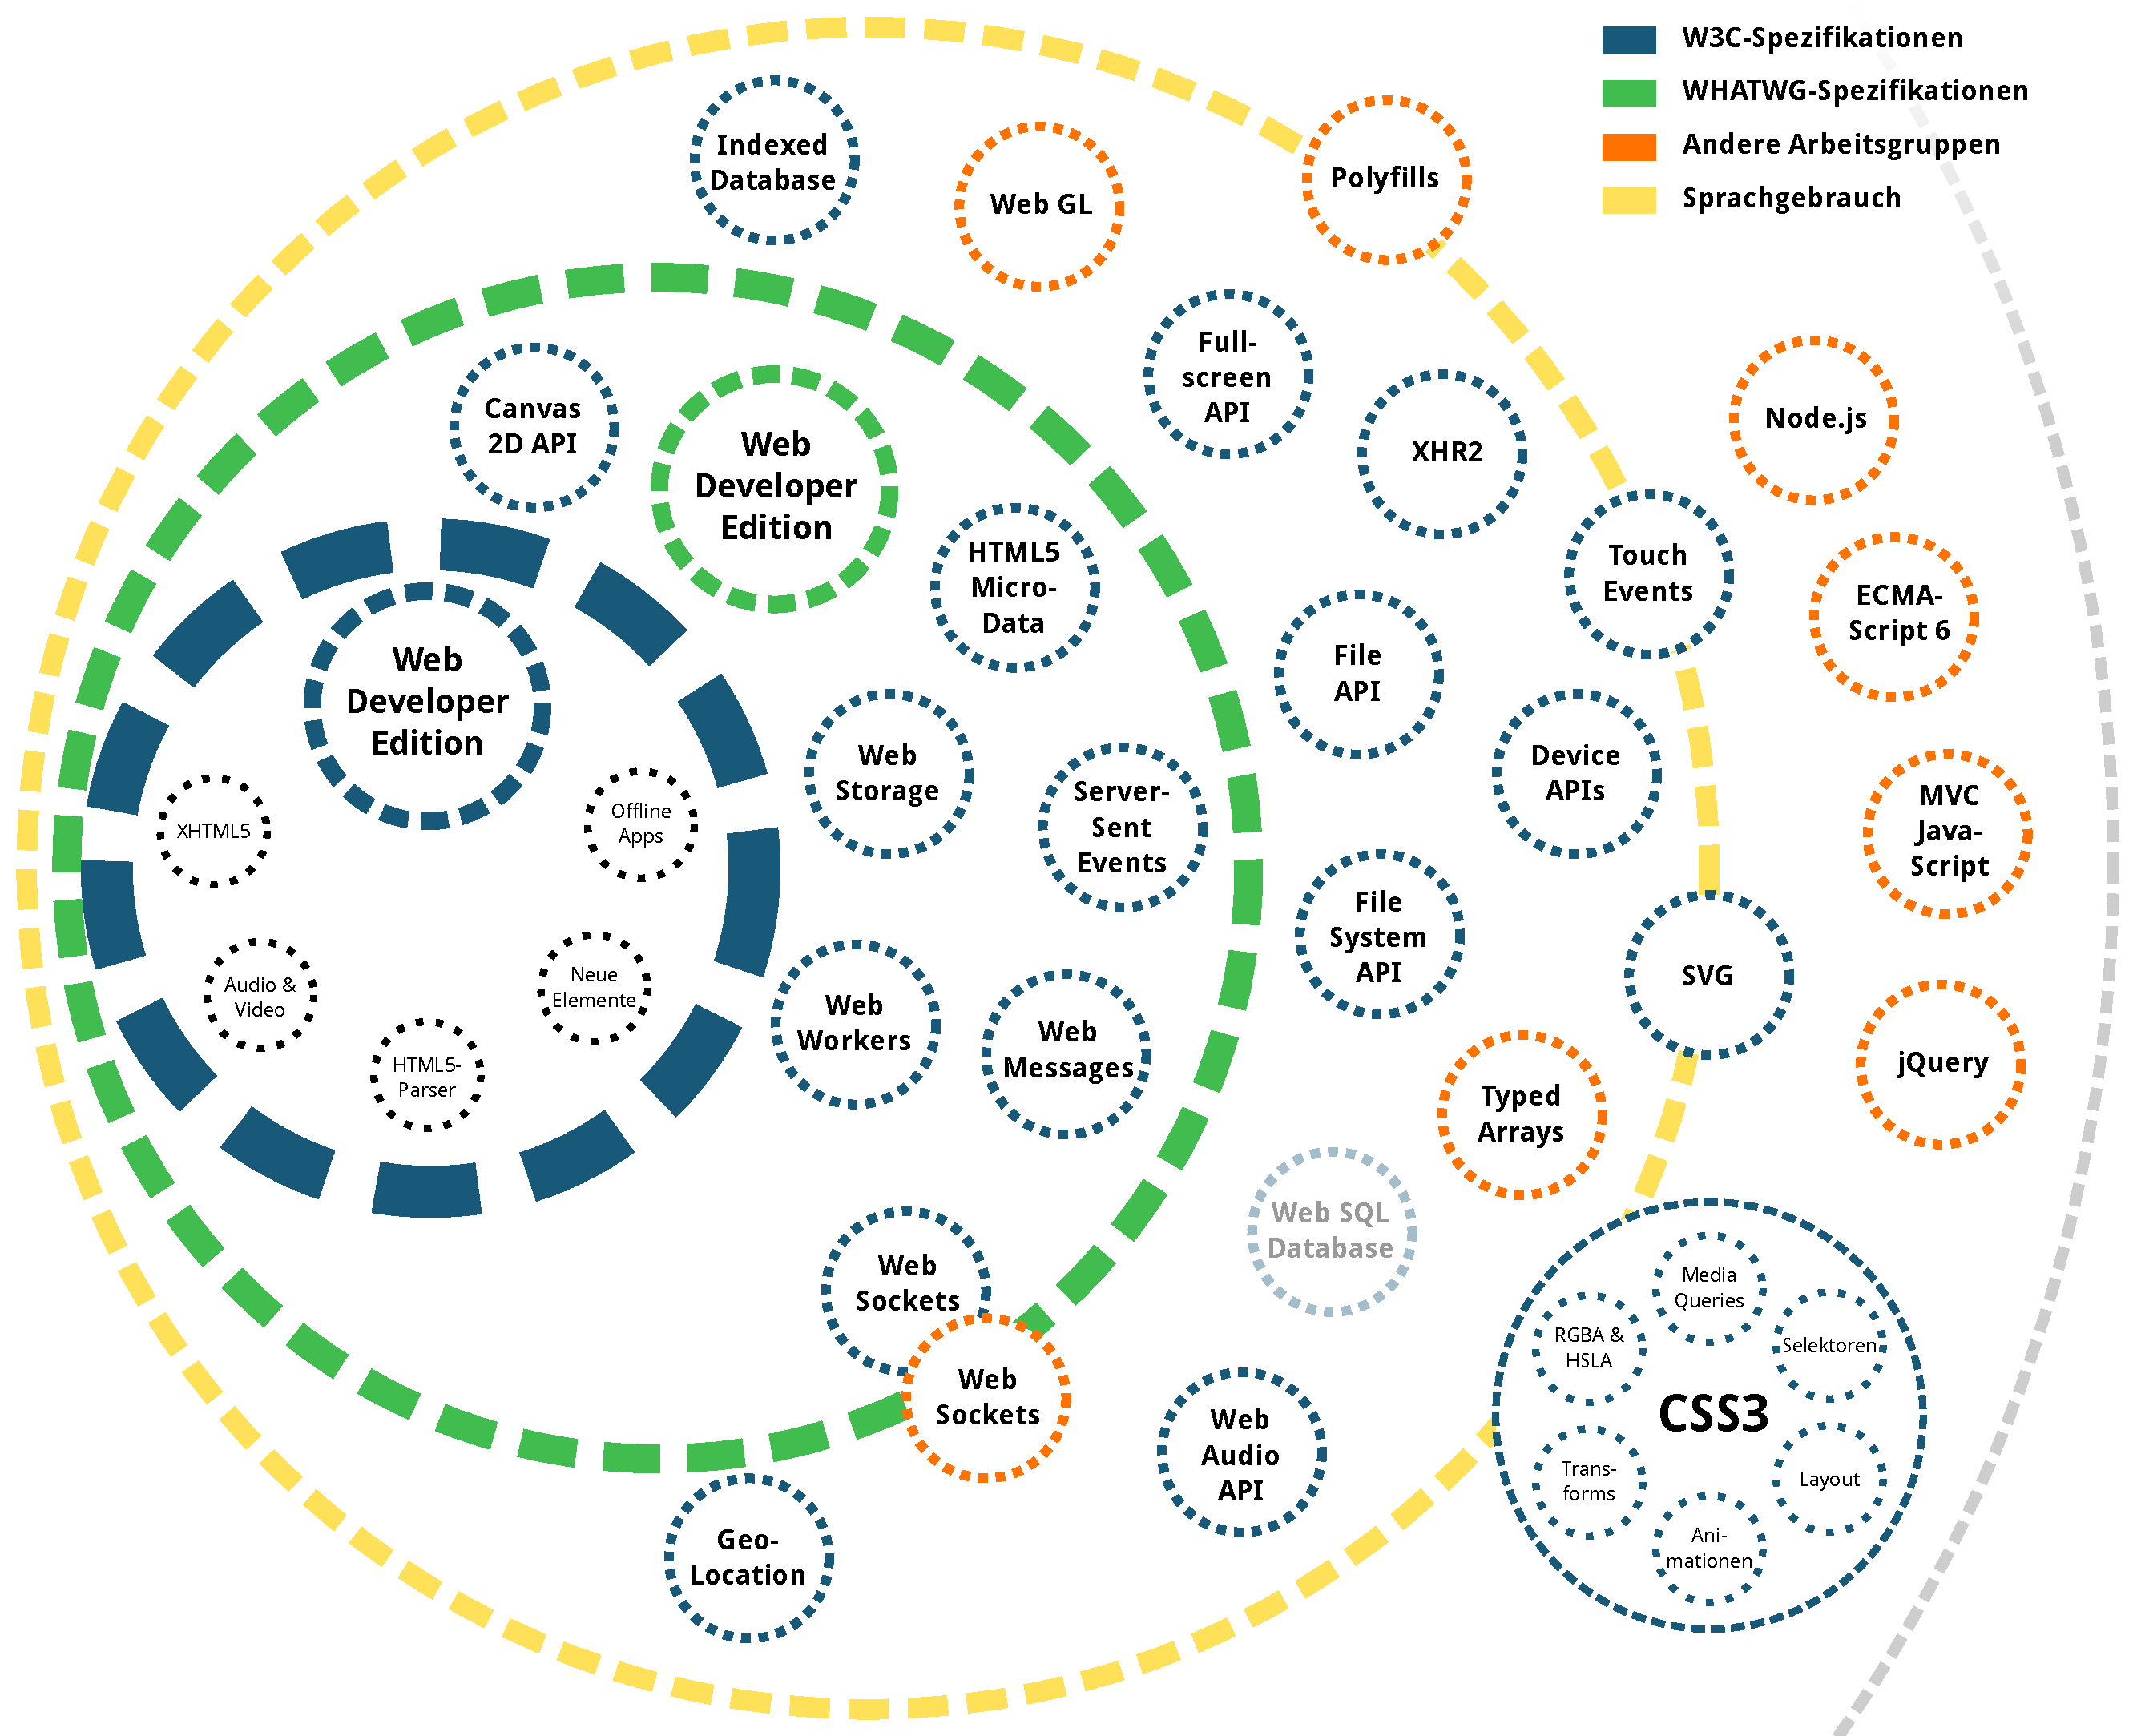
\includegraphics[width=\textwidth]{media/specGraph.pdf}
\caption{HTML5 Spezifikations-�bersicht (CC-BY-3.0 Peter Kr�ner) \cite{specGraph}}
\label{specgraphfig}
\end{figure}



Eine der Design-Entscheidungen bei der Entwicklung von HTML5 ist, den bestehenden Standard HTML 4.01 nicht zu ersetzen, sondern weiterzuentwickeln. Dadurch entsprechen die meisten Webseiten im HTML-4.01-Standard nach Anpassung der Dokumententypdeklaration direkt dem HTML5-Standard. \ref{diveInto}

Die Spezifikation hat den Status ``Last Call''\footnote{Stand: 22. August 2012}. Damit fordert das W3C auf letzte �nderungsvorschl�ge einzureichen, bevor der Standard im Jahr 2014 den Status ``Recommendation'' erhalten soll und damit final ist. Da jedoch die Implementierung in den einzelnen Browsern weit fortgeschritten ist und kaum noch �nderungen am Standard erwartet werden, kann er bereits jetzt eingesetzt werden. \cite{w3cpr}


\subsubsection{DOM und JavaScript APIs}

Nach dem parsen bildet der Browser intern die hierarchische Struktur eines HTML-Dokuments in Form eines Baumes ab. Diese Abbildung wird als \emph{Document Object Model (DOM)} bezeichnet. Der Zugriff auf den DOM-Baum ist mittels einer Schnittstelle (\emph{Application Programmable Interface (API)}) f�r JavaScript-Anwendungen m�glich. Elemente, Attribute und Texte sind als Knoten-Objekte angelegt und k�nnen ausgelesen oder manipuliert werden. \ref{mozdom}

Mit der zunehmenden Nutzung von Web-Applikationen sind auch die Anforderungen an die Browser gestiegen. Zur besseren Interaktion des Nutzers mit dem Browser wurden im Umfeld des HTML5-Standards viele weitere JavaScript-APIs definiert und vom W3C standardisiert (vgl. Abbildung \ref{specgraphfig}). \ref{keith} \ref{diveInto}



\subsubsection{Das canvas-Element}
\label{canvasapi}
Das \emph{canvas}-Element, wie in HTML5 definiert, ist ein rechteckiges Blockelement, das ohne weitere Anweisungen komplett unsichtbar ist: Es hat keinen sichtbaren Rahmen und der Inhalt des Elements ist transparent. In einem Dokument k�nnen sich beliebig viele canvas-Elemente befinden, die komplett unabh�ngig von einander sind. Jedes canvas ist im DOM-Baum verankert und kann mit einer ID versehen werden. Innerhalb des canvas-Elements kann alternativer Inhalt angegeben werden, der angezeigt wird wenn der Browser die Darstellung von canvas-Elementen nicht unterst�tzt. Eine beispielhafte Nutzung des Elements kann wie folgt aussehen: \ref{keith} \ref{diveInto}
\begin{verbatim}
    <canvas id="c" width="300" height="200">Fallback</canvas>
\end{verbatim}
Das Element definiert ein aufl�sungsabh�ngiges Bitmap, das in Echtzeit mit Grafikinhalten gef�llt werden kann. Laut Spezifikation definiert canvas einen JavaScript-Funktionsaufruf \verb+canvas.getContext(contextId [, ... ])+ bei dem ein Schl�sselwort in Form eines Strings als \verb+contextId+ �bergeben wird. \cite{W3Ccanvas} Die \emph{WHATWG} spezifiziert zwei m�gliche Kontexte: \verb+2d+ und \verb+webgl+. \cite{WHATWGcanvasContext} Der Funktionsaufruf liefert ein Objekt zur�ck das die jeweilige API bereitstellt oder \verb+null+ falls ein entsprechender Kontext nicht unterst�tzt wird.

Mittels der 2D-API k�nnen einfache Zeichenoperationen ausgef�hrt werden. Dazu geh�ren Linien, Pfade, Rechtecke, Ellipsen, aber auch Texte oder Bilder k�nnen eingef�gt werden. All diese Operationen werden direkt in der CPU berechnet und sind somit nicht hardwarebeschleunigt. Animationen k�nnen durch st�ndiges Neuzeichnen mittels JavaScript-Timer-Funktionen realisiert werden. \ref{WHATWGcanvas} \ref{diveInto}

\label{initwebgl}


% http://www.whatwg.org/specs/web-apps/current-work/multipage/the-canvas-element.html#drawing-text-to-the-canvas
% http://www.peterkroener.de/was-ist-html5-und-was-nicht-und-was-haette-der-kaiser-dazu-gesagt/
\chapter{Dreidimensionale Computergrafik im Browser}

\section{Historische Entwicklung der 3D-Technologie im Web}
\label{hist}

Erste Bem�hungen dreidimensionale Inhalte in den Webbrowser zu bringen begannen im Jahr 1994. Angelehnt an die Nutzung von HTML f�r die Darstellung von Webseiten sollte eine Auszeichnungssprache f�r die Darstellung dreidimensionaler Inhalte geschaffen werden. Anforderungen an die neue Sprache waren Plattformunabh�ngigkeit, Erweiterbarkeit und Nutzbarkeit auch bei geringer Internet-Bandbreite. Das zu diesem Zweck gegr�ndete \emph{Web3D}-Konsortium entwickelte die \emph{Virtual Reality Modeling Language (VRML)}. Am 26. Mai 1995 wurde die finale Spezifikation von \emph{VRML 1.0} ver�ffentlicht. Dort wird ein einfaches textbasiertes Format definiert, in dem Objekte geschachtelt abgelegt werden k�nnen. Diese Objekte k�nnen Kameras, Lichter, Materialien, aber auch dargestellte 3D-Objekte oder Transformationen sein. Zur Speicherung der Szenen wird die Dateiendung \verb+.wrl+ (f�r engl. \emph{world}) vorgegeben. \cite{vrml10} 1997 wurde \emph{VRML 2.0 (VRML97)} fertiggestellt und als ISO-Standard 14772-1:1997 definiert. Unter anderem wurde der VRML-1.0-Standard um Animationen und Nutzerinteraktionsm�glichkeiten erweitert. \cite{vrml97} \cite{vrml972}

F�r die Darstellung von VRML-Inhalten gibt es einige Browser-Plugins, jedoch integrierete nahezu kein Browser-Hersteller den Standard direkt in sein Produkt. In den folgenden Jahren entstanden viele weitere Dateiformate zur Speicherung von 3D-Szenen mit Augenmerk auf die Darstellung im Browser. Unter anderem trat das XML-basierte Format \emph{X3D} die Nachfolge von VRML an. Das Web3D-Konsortium schl�gt vor den X3D-Standard komplett in HTML5 zu integrieren, jedoch hat das W3C das bisher abgelehnt: \emph{``Embedding 3D imagery into XHTML documents is the domain of X3D, or technologies based on X3D that are namespace-aware.''} \cite{nox3d} �hnlich wie bei \emph{SVG} oder \emph{MathML} soll so eine native Darstellung ohne Plugin erm�glicht werden. \cite{x3domhtml}



\section{Deklarative und imperative 3D-Darstellung in Browsern}


Die Darstellung von zwei- und dreidimensionalen Grafiken im Browser kann grundlegend auf zwei verschiedene Arten erfolgen: Zum einen ist es m�glich den Szenengraph als Teil des HTML-Dokuments zu deklarieren. Somit sind die einzelnen Objekte der Grafik gleichberechtigt mit HTML-Elementen auf der Seite. Jedes Objekt der Grafik ist im DOM-Baum integriert und kann per CSS oder JavaScript selektiert und modifiziert werden. Zur Darstellung zweidimensionaler Grafiken ist das \emph{SVG}-Format im HTML5-Standard aufgenommen. Das �quivalent f�r dreidimensionale Grafiken, X3D, ist wie in Kapitel \ref{hist} beschreiben nicht Teil des Standards. \cite{x3dom} 

Zum anderen k�nnen Grafiken imperativ auf eine Zeichenfl�che gezeichnet werden. Als Zeichenfl�che wird das canvas-Element genutzt und ist dabei das einzige Objekt der Grafik, das im DOM-Baum verankert ist. Inhalte die auf die Zeichenfl�che gezeichnet wurden k�nnen nicht mehr ver�ndert werden. Die Zeichenfl�che kann lediglich komplett oder in Ausschnitten geleert und/oder �berzeichnet werden. HTML5 definiert die 2D-F�higkeiten des canvas-Elements und Verwendung von WebGL f�r 3D-Inhalte. \cite{2dcontext}

\begin{table}[h]

\centering
\begin{tabular}{l||c|c}
     & \textbf{2D} & \textbf{3D} \\
\hline
\hline
    \textbf{Deklarativ} & SVG & X3D\footnotemark \\
\hline
    \textbf{Imperativ} & canvas & WebGL
\end{tabular}

\label{tbl:tablelabel}
\caption{Deklarative und imperative Grafikdarstellung im Web \cite{x3dom}}
\end{table}
\footnotetext{nicht vom W3C standardisiert}

%http://www.w3.org/TR/2dcontext/



\chapter{WebGL}


Die \emph{Khronos Group} ist ein Konsortium aus �ber 100 Firmen, die es sich seit Januar 2000 zum Ziel gesetzt hat, offene Standards f�r Mediendarstellung auf Computern, mobilen Ger�ten und in integrierten Systemen zu definieren. Als gemeinn�tzige Organisation arbeitet die Gruppe nicht gewinnorientiert und finanziert sich lediglich aus den j�hrlichen Beitr�gen ihrer Mitglieder. In verschiedenen Arbeitsgruppen sollen Industrie-Standards entwickelt und linzenzfrei zur Verf�gung gestellt werden. Dazu gibt es das \emph{Khronos IP Framework}--eine Vereinbarung zwischen den Khronos-Mitgliedern, keine Patentstreitigkeiten bez�glich der Khronos-Standards gerichtlich auszutragen. \cite{KhronosAbout}

Der �lteste Standard der Khronos-Gruppe ist \emph{OpenGL (Open Graphics Library)}, der 1992 von \emph{Silicon Graphics Inc. (SGI)} entwickelt wurde. OpenGL spezifiziert eine hardwareunabh�ngige Software-Schnittstelle (API) zum Grafikprozessor mit mehreren hundert Befehlen, einer kleinen Menge geometrischer Primitive und einer eigenen Shader-Programmiersprache \emph{OpenGL Shading Language (GLSL)}. Die meisten gro�en Betriebssysteme, darunter Windows, Mac OS und Linux, unterst�tzen OpenGL. \cite{Shreiner} \cite{SGI} \cite{KhronosAbout2}

Als propriet�re Alternative zu OpenGL bietet Microsoft \emph{Direct3D} f�r die Windows- und XBox-Plattform an. Zudem gibt es eine angepassten Version f�r Microsofts mobiles Betriebssystem \emph{Windows Phone Series}.

Ausgehend vom OpenGL-Standard entwickelte die Khronos Group einen weiteren Standard: \emph{OpenGL for Embedded Systems (OpenGL ES)} ist eine Teilmenge von OpenGL, die speziell f�r den Einsatz auf mobilen Ger�ten wie etwa Smartphones oder Spielekonsolen entwickelt wurde und eine hohe Verbreitung unter anderem in Googles Android \cite{devGoogle} oder Apples iOS \cite{devApple} findet. Applikationen die gegen OpenGL ES geschrieben wurden laufen auch unter der entsprechenden Version von OpenGL. Andersherum ist das nicht der Fall.


WebGL bringt nun die M�glichkeit OpenGL-ES-2.0-Inhalte im Browser darzustellen und dabei die Hardware-Beschleunigung der Grafikkarte zu nutzen. Bisher konnten Webinhalte lediglich den Hauptprozessor (CPU) f�r ihre Berechnungen nutzen. Grafikkarten sind hochgradig f�r die typischen Berechnungen von 3D-Darstellungen optimiert und k�nnen die Prozessorleistung bei weitem �bertreffen. Mittels der WebGL-Technologie k�nnen Applikationen die zum Beispiel f�r mobile Ger�te konzipiert wurden ohne gr��ere Anpassungen im Browser ausgef�hrt werden. Die Anwendungsgebiete sind vielf�ltig: Von Visualisierungen, Simulationen, Spielen, bis zu Kunst ist alles denkbar. \cite{operawebgl} \cite{webgl}


\section{Technik und Funktionsumfang}
\label{tecandfunc}
Die WebGL-Programmierung erfolgt in JavaScript und die Programmierung der Shader in GLSL, deren Syntax �hnlich zu JavaScript ist. Shader sind das grundlegende Konzept von WebGL und OpenGL. Dabei handelt es sich um Unterprogramme, die in der Grafikkarte ausgef�hrt werden und �ber die Darstellung der 3D-Szene entscheiden. In WebGL gibt es mit Vertex- und Fragment-Shader zwei unterschiedliche Arten, deren Funktionsweise in Kapitel \ref{pipeline} erl�utert wird. Die Shader k�nnen frei programmiert werden, aber viele Grafikbibliotheken bringen bereits vordefinierte Shader mit (vgl. Kapitel \ref{webglbib}).

Das canvas-Element wird als Zeichenfl�che f�r die WebGL-Inhalte verwendet. Wie jedes andere HTML-Element kann das canvas-Element �ber oder unter anderen Elementen des Dokuments dargestellt werden. So ist auch die �berlagerung von HTML- und WebGL-Inhalten m�glich.

Mittels des in Kapitel \ref{initwebgl} beschriebenen Funktionsaufrufs kann die Initialisierung eines WebGL-Kontexts wie Listing \ref{webglinitcode} aussehen. \cite{html5rocks} Zun�chst wird der Funktionsaufruf der Initialisierung auf den \verb+onload+-Event-Listener gelegt (Zeile \verb+11+) und somit die Funktion \verb+init()+ beim Laden der Seite aufgerufen. Mittels der Element-ID wird das canvas-Element selektiert (Zeile \verb+3+) und dessen WebGL-Kontext aufgerufen (Zeile \verb+4+). Ist der Kontext nicht vorhanden, wird WebGL nicht unterst�tzt (Zeilen \verb+5+-\verb+7+), andernfalls steht dann der WebGL-Kontext �ber die Variable \verb+gl+ zur Verf�gung.

\begin{lstlisting}[caption=Initialisierung eines WebGL-Kontexts,label=webglinitcode]
<script type="text/javascript">
    function init() {
        canvas = document.getElementById("c");
        gl = canvas.getContext("webgl");
        if (!gl) {
            return; /*WebGL wird nicht unterst�tzt*/
        }
        ...
    }

    window.onload = init;
</script>
<canvas id="c"></canvas>
\end{lstlisting} 

Zus�tzlich k�nnen Vertex- und Fragment-Shader mit folgendem Mark-Up ausgezeichnet werden und dann in GLSL programmiert werden:

\begin{lstlisting}[caption=Deklaration der WebGL-Shader]
<script id="vshader" type="x-shader/x-vertex">
    ... /* Vertex-Shader */
</script>
<script id="fshader" type="x-shader/x-fragment">
    ... /* Fragment-Shader */
</script>
\end{lstlisting} 

WebGL verwendet ein eigenes kartesisches Koordinatensystem das unabh�ngig von der Gr��e und Aufl�sung des canvas-Elements ist. Der Wertebereich der x-, y- und z-Achse liegt im Intervall $[-1;1]$. Die x-Achse beginnt auf der linken Seite mit $-1$, die y-Achse hat den Wert $-1$ an der unteren Bildkante. Die z-Ache zur Tiefenbestimmung hat f�r die n�chsten Objekte den Wert $-1$ und f�r die entferntesten den Wert $1$. F�r die Darstellung auf dem Bildschrim werden die WebGL-Koordinaten dann auf die canvas-Koordinaten umgerechnet.


\subsection{Die WebGL-Rendering-Pipeline}
\label{pipeline}
Folgende Schritte werden bei der Berechnung eines Bilds bei der OpenGL-ES-/WebGL-Technologie durchlaufen. Der Ablauf ist vereinfacht dargestellt und weitaus identisch mit der Arbeitsweise anderer Grafik-Bibliotheken. \cite{beginnersGuide} \cite{operawebgl} \cite{Shreiner}

\begin{enumerate}
    \item Wie f�r 3D-Renderingprozesse �blich, verwendet WebGL polygonale Modellierung. Das bedeutet, dass Objekte aus Polygonen zusammengesetzt werden. �blicherweise und auch in WebGL werden daf�r Dreiecke verwendet. In JavaScript-Code wird nun eine Menge von Punkten (Vertices) definiert und in einem Array gespeichert. Zu jedem Vertex k�nnen neben der Position im dreidimensionalen Raum auch die Farbe, Transparenz und Texturkoordinaten gespeichert werden. Ein zweites Array ordnet die Indizes des Vertex-Arrays zu Dreiergruppen zusammen und gibt die Reihenfolge an, in der die Punkte zu Dreiecken zusammengesetzt werden.
    
    \item Das Vertex- und Index-Array werden dann an die Grafikkarte �bergeben. F�r jedes Vertex wird ein Unterprogramm, der so genannte \textbf{Vertex-Shader}, aufgerufen, der Operationen auf jedem einzelnen Vertex ausf�hren kann. Hier k�nnen Manipulationen an den Formen des Objekts vorgenommen werden. Au�erdem wird mit Hilfe einer Matrixmultiplikation die Projektion des dreidimensionalen Punkts auf die zweidimensionale Fl�che zur Anzeige auf dem Bildschirm berechnet. 
        
    \item Anschlie�end wird in der Grafikkarte das Bild \textbf{rasterisiert}. Dabei wird die zweidimensionale Projektion mit einem Pixelraster der Gr��e des canvas-Elements �berlagert und jeder Punkt einem Pixel zugeordnet. Hier k�nnen auch Kantengl�ttungs-Mechanismen (Antialiasing) angewendet werden. Die Farben zwischen zwei Vertices k�nnen mit Hilfe der zugeh�rigen Farbwerte interpoliert werden.
    
    \item F�r jedes berechnete Pixel wird nun ein weiteres Unterprogramm aufgerufen: Der \textbf{Fragment-Shader} kann die Farbewerte des jeweiligen Pixels ver�ndern und sorgt somit f�r die Darstellung von Texturen, Oberfl�chenmaterialien, Lichtern und Schatten.
    
    \item Das fertige Pixelbild wird im \textbf{Frame-Buffer} der Grafikkarte abgelegt und kann von dort aus dann im canvas-Element der Webseite dargestellt werden.
\end{enumerate}


\section{Verbreitung und Implementierung in den verschiedenen Browsern}

Mitglieder der Khronos Group sind mit Google (Chrome), Apple (Safari), Mozilla (Firefox) und Opera unter anderem einige namenhafte Browser-Hersteller, die gemeinsam an der Entwicklung von WebGL arbeiten. Deshalb geschieht die Adaption neuer Funktionen in den genannten Browsern meist schnell und fl�chendeckend.

\subsection{Vergleich der WebGL-F�higkeiten ausgew�hlter Browser}

F�r den Vergleich wurden die f�nf Browser mit den gr��ten Marktanteilen herangezogen. Gemeinsam decken diese f�nf Browser 98,41\%\footnote{Stand: Juli 2012} des Desktop-Marktes ab. \cite{StatTop5Browser} Mobile Browser sind in diesem Vergleich ausgenommen und werden gesondert in Kapitel \ref{mobilewebGL} behandelt. 

Der \emph{WHATWG}-Standard \cite{WHATWGcanvas} gibt f�r den Aufruf der Schnittstelle des WebGL-Kontexts das Schl�sselwort \verb+webgl+ vor, jedoch implementieren die verglichenen Browser alle ausschlie�lich das Schl�sselwort \verb+experimental-webgl+ und liefern f�r den Kontext \verb+webgl+ den Wert \verb+null+ zur�ck.\footnote{Stand: August 2012 (Chrome 21, Firefox 14, Safari 6.0, Opera 12.00)} Solange die Spezifikation nicht final ist und der Standard nicht vollst�ndig implementiert wurde wird dieses Vorgehen vom \emph{W3C} und der \emph{WHATWG} empfohlen. \cite{W3Ccanvas} \cite{WHATWGcanvas}


\subsubsection{Microsoft Internet Explorer}

Microsoft stuft die Implementierung von WebGL als zu gef�hrlich ein und verzichtet deshalb auf eine Integration in den \emph{Internet Explorer}. Problematisch sieht Microsoft dabei die direkte Bereitstellung der Grafikkarte f�r beliebige Webseiten-Betreiber. Sicherheitsl�cken in Grafikkarten-Treibern die bisher nur lokal ausgenutzt werden konnten, stehen somit f�r das Internet offen (vgl. Kapitel \ref{webglsec}). \cite{MSWebGL} Als alternative Technologie schl�gt Microsoft die Eigenentwicklung \emph{Silverlight} vor, die seit der Version 5 ebenfalls hardwarebeschleunigte 3D-Darstellung unterst�tzt. \cite{Silverlight}

Dennoch l�sst sich mittels Plugin eines Fremdanbieters die Unterst�tzung f�r WebGL ab Internet Explorer Version 8 nachr�sten. \cite{IEWebGL}




\subsection{Marktanteile der Webbrowser}

\begin{table}[h]

\centering
\begin{tabular}{l|rrcr}
    \textbf{Browser} &   \vbox{\hbox{\strut \textbf{Marktanteil}}\hbox{\strut \verb+     +\textbf{gesamt}}} & \vbox{\hbox{\strut \textbf{WebGL ab}}\hbox{\strut \verb+  +\textbf{Version}\footnotemark}} & \textbf{Release} & \vbox{\hbox{\strut \verb+ +\textbf{Marktanteil}}\hbox{\strut \textbf{WebGL-f�hig}}}\\
\hline
\hline
    Google Chrome & 33,29\% & 9.0 & 03.02.2011 \cite{releaseChrome} & 32,89\% \\
\hline
    Internet Explorer & 32,17\% &\multicolumn{2}{r}{\textit{keine WebGL Unterst�tzung}} & 0,00\% \\
\hline
    Mozilla Firefox & 24,14\% & 4.0 & 22.03.2011 \cite{releaseFirefox} & 22,13\%\\
\hline
    Apple Safari & 7,06\% & 5.1 & 20.07.2011 \cite{releaseSafari} & 3,41\%\\
\hline
    Opera & 1,75\% & 12.00 & 14.06.2012 \cite{releaseOpera} & 0,78\%\\
\hline
\hline
    \textbf{Summe} & \textbf{98,41\%} & & & \textbf{59,21\%} \\
\end{tabular}

\caption{Marktanteile der f�hrenden Webbrowser\cite{StatTop5Browser} \cite{statVersion}}
\label{marketshare}
\end{table}

\footnotetext{F�r den Vergleich wurden nur finale Versionen der jeweiligen Browser herangezogen. Alpha-, Beta- und Preview-Versionen sind ausgenommen und waren teilweise schon wesentlich fr�her verf�gbar.}


Basierend auf den Zahlen von StatCounter.com f�r Juni bis Juli 2012 haben WebGL-f�hige Browserversionen einen Marktanteil von 59,21\% (vgl. Tabelle \ref{marketshare}). Jedoch muss der Anteil der Browser, die WebGL-Inhalte korrekt darstellen geringer angegeben werden, da durch Inkompatibilit�ten mit speziellen Grafikkarten einige Browserversionen WebGL deaktivieren. Hinzu kommt, dass Safari mit deaktiviertem WebGL ausgeliefert wird, welches erst vom Benutzer manuell aktiviert werden muss. Daher lassen sich ohne eigener Erhebung dieser Daten keine verl�sslichen Aussagen �ber die genaue Verbreitung von Browsern mit aktivierter WebGL-F�higkeit treffen.




\subsection{Mobile Verf�gbarkeit von WebGL} \label{mobilewebGL}

Es wurde die Verf�gbarkeit des WebGL-Standards auf den beiden f�hrenden mobilen Betriebssystemen verglichen. \cite{mobileos} Dabei wird die grundlegende Verf�gbarkeit der OpenGL-Technologie sowie die Implementierung der WebGL-Technologie im mitgelieferten Browser betrachtet. 

\subsubsection{Apple iOS und Mobile Safari}

Apple implementiert in iOS\footnote{Stand: iOS 5.1.1} OpenGL ES 1.1 und 2.0 f�r die Darstellung von 2D- und 3D-Inhalten. Applikationsentwickler k�nnen die Standards f�r die Darstellung ihrer Inhalte nutzen. \cite{iosopengl} Jedoch ist die Nutzung von OpenGL in Form von WebGL im systemeigenen Browser \emph{Mobile Safari} nicht m�glich. F�r in Applikationen eingebettete Web-Darstellungen l�sst sich WebGL aktivieren, jedoch widerspricht die Nutzung Apples Richtlinien f�r Entwickler. Lediglich innerhalb Apples webbasiertem Werbenetzwerk \emph{iAd} ist die Nutzung von WebGL m�glich. Au�erdem kann die Darstellung von \emph{CSS3-Animationen} im Browser auf Hardwarebeschleunigung zur�ckgreifen. \cite{devApple}

\subsubsection{Android}

F�r die Entwicklung von Applikationen unterst�tzt die Android-Plattform ebenso den OpenGL ES 1.1 und ab Android 2.2 (API Level 8) auch den OpenGL ES 2.0 Standard. \cite{devGoogle} WebGL ist im Android Browser nicht verf�gbar. Sony entwickelte eine Modifikation f�r den Android Browser die WebGL implementiert. \cite{sonywebgl} Diese wird bisher nur auf dem \emph{Sony Xperia} Smartphone eingesetzt.

\section{Sicherheit in WebGL}
\label{webglsec}

Im Mai 2011 beschrieb \emph{Context Information Security} mehrere m�gliche Angriffsszenarien mit Hilfe von manipulierten WebGL-Inhalten. \cite{contextwebgl} Generell stellt WebGL ein hohes Bedrohungspotential dar, da es den direkten Zugriff von Webseiten auf die Hardware des Rechners zul�sst. Nat�rlich versuchen Browserhersteller, die Khronos Group und die Grafikkartenhersteller diese Angriffe zu verhindern, trotzdem sind diverse Szenarien denkbar, in denen WebGL dazu genutzt werden kann den Rechner anzugreifen.

\subsection{Denial-of-Service-Attacken}

Mittels sehr komplexer 3D-Geometrien oder extrem aufw�ndiger Shaderprogramme wird die Grafikkarte so lange beansprucht, dass weder andere Programme noch das Betriebssystem die Grafikkarte nutzen k�nnen und der Rechner so unter Umst�nden abst�rzt oder unbenutzbar wird. \cite{contextwebgl2} Gegen diese Art von Angriff wurden bisher kaum Ma�nahmen ergriffen. Seit Windows Vista implementiert Microsoft einen Sicherheitsmechaniasmus, der die Grafikkarte zur�cksetzt, wenn diese f�r �ber zwei Sekunden nicht mehr reagiert. \cite{windows} Dieses Vorgehen schl�gt auch die Khronos Group f�r OpenGL-kompatible Grafikkarten in der Erweiterung \emph{GL\_ARB\_robustness} vor, jedoch haben noch nicht alle Grafikkartenhersteller diese Erweiterung implementiert. Somit sind aktuell viele System f�r diese Art von Angriff gef�hrdet. \cite{KhrSec}

% http://msdn.microsoft.com/en-us/windows/hardware/gg487368.aspx
% http://www.khronos.org/news/permalink/webgl-security

\subsection{Zugriff auf den Frame-Buffer}

Die WebGL-Technologie erm�glicht Webseiten den Zugriff auf den Inhalt des Frame-Buffers der Grafikkarte. Der Frame-Buffer ist ein gemeinsam genutzter Speicherbereich in dem alle auf dem Bildschirm dargestellten Inhalte liegen. Deshalb ist laut Spezifikation der Zugriff auf den Teil des Frame-Buffers beschr�nkt, der den Inhalt des canvas-Elements speichert. Jedoch kam es durch fehlerhafte Implementierungen des WebGL-Standards und Bugs in Grafikkarten-Treibern dazu, dass auch andere Inhalte des Frame-Buffers in das canvas-Element gezeichnet werden konnten. So konnten Informationen ausgelesen werden, die der Nutzer beispielsweise in anderen Applikationen oder auf seinem Desktop dargestellt hat. Seitens Khronos Group un der Grafikkartenhersteller wurden diese Fehler behoben. Es ist jedoch nicht ausgeschlossen, dass durch neue Sicherheitsl�cken dieser Angriff wieder erm�glicht wird. \cite{contextwebgl2}

\subsection{Cross-Domain Texturen}

Das Nachladen externer Modelle oder Texturen kann den Zugriff auf fremde Ressourcen erfordern. Ein Sicherheitskonzept, das mit \emph{Netscape Navigator 2.0} f�r clientseitige Skriptsprachen, wie beispielsweise JavaScript, eingef�hrt wurde ist die \emph{Same-Origin-Policy (SOP)}. Diese verbietet clientseitige lesende Zugriffe, zum Beispiel per \emph{XMLHttpRequest}, auf fremde Ressourcen. Sie verlangt, dass Zugriffe innerhalb einer Webseite nur auf Ressourcen der selben Domain, �ber den selben Port mittels des selben Protokolls erfolgen d�rfen. Das betrifft nicht das Einbinden fremder Inhalte, wie das Einbetten eines Bildes, sondern den lesenden Zugriff eines Skripts auf solche Inhalte. Durch einen clientseitigen lesenden Zugriff k�nnten Informationen von fremden Seiten ausgelesen werden. H�tte ein Nutzer beispielsweise eine Banking-Seite ge�ffnet, k�nnte eine andere Seite deren Inhalte einlesen und zu einem fremden Server �bertragen. Daher wird der clientseitige lesende Zugriff im Normalfall auf die jeweilige Domain beschr�nkt. \cite{MDNsop}

Um dennoch entfernte Ressoucen nutzen zu k�nnen wurde \emph{Cross-Origin-Resource-Sharing (CORS)} entwickelt. Dabei gibt der ausliefernde Server in seinem HTTP-Header an, welche fremden Seiten seine Ressourcen lesen d�rfen. Dabei ist auch die Verwendung einer Wildcard m�glich um den lesenden Zugriff f�r alle fremden Seiten zuerm�glichen. \cite{cors} \cite{corsbug}




\section{WebGL-Bibliotheken}
\label{webglbib}
Um den Umgang mit WebGL zu vereinfachen gibt es einige Bibliotheken. Diese stellen beispielsweise geometrische Grundformen wie W�rfel, Kugeln, Zylinder, etc. zur Verf�gung. Au�erdem lassen sich somit WebGL-Aufrufe mittels JavaScript ausf�hren, ohne eigenen Shader-Code in \emph{GLSL} nutzen zu m�ssen. Komplexe mathematische Berechnungen die f�r die Realisierung verschiedener Kameras m�ssen nicht in einem eigenen Vertex-Shader realisiert werden, sondern k�nnen als fertige Programme geladen werden. Ebenso ist f�r die Realisierung von Oberfl�chenmaterialen und Beleuchtungsmodellen keine Programmierung eines eigenen Fragment-Shaders n�tig, da g�ngige Materialien und Beleuchtungsmodelle bereits als vordefinierte Shader vorhanden sind. F�r die meisten Anwendungsf�lle reicht die Nutzung der durch Kamera-, Material- und Beleuchtungsobjekten vordefinierten Shader aus und es muss kein Shadercode geschrieben werden. Die Programmierung kann dann ausschlie�lich in JavaScript erfolgen. Zus�tzlich k�nnen unterschiedliche Implementierungen verschiedener Browser angefangen und f�r den Programmierer unsichtbar gemacht werden.

\subsection{die THREE.js-Bibliothek}

Entwickelt von \emph{Ricardo Cabello Miguel} ist \emph{THREE.js} eine der am weitesten verbreiteten Bibliotheken f�r WebGL. Seit 2010 wird THREE.js entwickelt und befindet sich aktuell in der Version r50\footnote{Stand: 19. August 2012}. Einige elementare Bestandteile der Bibliothek sollen im Folgenden vorgestellt werden. \cite{threejsdocs}

\begin{itemize}
\item \textbf{Renderer:} Neben der Ausgabe in den \verb+webgl+-Kontext, ist in einem begrenzen Ma�e auch die Ausgabe in eine \emph{SVG}-Datei, oder in den \verb+2d+-Kontext des canvas-Elements m�glich. Jedoch ist nur die WebGL-Ausgabe hardwarebeschleunigt. F�r nicht WebGL-f�hige Browser kann in einigen Anwendungsf�llen eine der alternativen Ausgaben genutzt werden.

\item \textbf{Kameras:} THREE.js hat zwei verschiedene Kamera-Objekte zur Verf�gung. Eine orthographische Kamera die eine parallele Projektion auf die Sichtebene vornimmt, sowie eine persketivische Kamera, die dem Verhalten des menschlichen Auge entspricht. Hierbei wird das Sichtfeld mit einem Winkel angegeben.

\item \textbf{Geometische Primitive:} Einige geometische Primitive sind in der Bibliothek bereits angelegt und k�nnen verwendet werden. Darunter befinden sich: W�rfel, Zylinder, Ebene, Kugel und Torus.

\item \textbf{Lichter:} In THREE.js sind verschiedene Lichter definiert, die sich unterschiedlich auf die Szene auswirken. Das \verb+AmbientLight+ hellt die gesamte Szene auf, hat keine Richtung und wirft keine Schatten. Das \verb+DirectionalLight+ ist gerichtet, hat aber keinen Ursprung. Das Licht verl�uft parallel und wirft Schatten. \verb+SpotLight+ und \verb+PointLight+ haben eine punktf�rmige Position. Beide strahlen das Licht kugelf�rmig ab, wobei es linear abgeschw�cht wird. Nur SpotLights k�nnen Schatten werfen. 

\item \textbf{Oberfl�chenmaterialien:} Die unterschiedlichen Oberfl�chenmaterialien wirken sich auf das Verhalten von Licht auf den Objekten aus. Das \verb+BasicMaterial+ ignoriert einfallendes Licht und stellt das Objekt gleichm��ig in der angegebenen Farbe dar. F�r die realistische Darstellung bieten sich \verb+PhongMaterial+ und \verb+LambertMaterial+ an, die einfallendes Licht nach den jeweiligen Beleuchtungsmodellen verarbeiten und so die Farbdarstellung berechnen. Zus�tzlich ist es m�glich Grafiktexturen auf Objekten abzubilden.


\end{itemize}












%______________________________________________________________________

\cleardoublepage
\fancyhead[LE,RO,LO,RE]{} % Keine Kopfzeile mehr oben auf jeder Seite
\section*{Inhalt der beigelegten CD}
%______________________________________________________________________

\cleardoublepage
\begin{thebibliography}{99}


\bibitem[Kei10]{keith}
    \textbf{HTML5 for Web Designers} \\
    \textit{Jeremy Keith} \\
    A Book Apart, 2010

\bibitem[Pil10]{diveInto}
    \textbf{Dive into HTML5}  \\
    \textit{Mark Pilgrim}, 2010 \\

\bibitem[CB97]{vrml972}
    \textbf{The Annotated VRML 97 Reference Manual} \\
    \textit{Rikk Carey, Gavin Bell} \\
    Addison-Wesley Professional, 1997


\bibitem[Shr09]{Shreiner}
    \textbf{OpenGL Programming Guide} (Seventh Edition) \\
    \textit{Dave Shreiner} \\
    Addison-Wesley Longman, 2009

\bibitem[CJ12]{beginnersGuide}
    \textbf{WebGL Beginner's Guide}  \\
    \textit{Diego Cantor, Brandon Jones} \\
    Packt Publishing, 2012
    
\bibitem[Isi12]{Isi12}
    \textbf{SumoViz, HTML5-based Visualization of Pedestrian Simulation Data} \\
    \textit{Mustafa K. Isik} \\
    TU M�nchen, 10. Mai 2012

\bibitem[ALS10]{ALS10}
    \textbf{CouchDB: The Definitive Guide} \\
    \textit{J. Chris Anderson, Jan Lehnardt, Noah Slater} \\
    O'Reilly, 2010
    
\bibitem[Hol11]{Hol11}
    \textbf{Writing and Querying MapReduce Views in CouchDB} \\
    \textit{Bradley Holt} \\
    O'Reilly, 2011
    
\bibitem[McL11]{McL11}
    \textbf{What Is Node?} \\
    \textit{Brett McLaughlin} \\
    O'Reilly, 2011
    
\bibitem[Fla06]{Fla06}
    \textbf{JavaScript: The Definitive Guide} \\
    \textit{David Flanagan} \\
    O'Reilly, 2006
    
    
\cleardoublepage
\hspace{-\leftmargin}{\Large\bfseries Web-Referenzen} % W�ster Hack %-|



\bibitem[Tre11]{KhronosAbout}
    Neil Trevett: Building Markets for Advanced Devices through Open Standards \\
    \url{http://www.khronos.org/assets/uploads/developers/library/overview/khronos_overview.pdf}, abgerufen am 18.08.2012.

\bibitem[SGI]{SGI}
    SGI: OpenGL \\
    \url{http://www.sgi.com/products/software/opengl/?/overview.html}, \\ abgerufen am 18.08.2012.

\bibitem[Khr]{KhronosAbout2}
    About The Khronos Group \\
    \url{http://www.khronos.org/about}, abgerufen am 18.08.2012.

\bibitem[Goo]{devGoogle}
    Android Developers: Andriod 2.2 APIs \\
    \url{http://developer.android.com/about/versions/android-2.2.html}, \\ abgerufen am 18.08.2012.

\bibitem[App]{devApple}
    OpenGL ES for iOS \\
    \url{https://developer.apple.com/devcenter/ios/resources/opengl-es/}, \\ abgerufen am 18.08.2012.
    
\bibitem[Cab]{operawebgl}
    Luz Caballero (Opera): An introduction to WebGL \\
    \url{http://dev.opera.com/articles/view/an-introduction-to-webgl/}, \\ abgerufen am 18.08.2012.
        
\bibitem[Ope]{webgl}
    Khronos Group: WebGL - OpenGL ES 2.0 for the Web \\
    \url{https://www.khronos.org/webgl/}, abgerufen am 18.08.2012.
    
\bibitem[W3c]{W3Ccanvas}
    W3C: HTML5, The canvas element \\
    \url{http://www.w3.org/TR/html5/the-canvas-element.html#the-canvas-element}, \\ abgerufen am 18.08.2012.

\bibitem[WHc]{WHATWGcanvasContext}
    WHATWG: CanvasContexts \\
    \url{http://wiki.whatwg.org/wiki/CanvasContexts}, abgerufen am 18.08.2012.

\bibitem[Whc2]{WHATWGcanvas}
    WHATWG: The canvas element \\
    \url{http://www.whatwg.org/specs/web-apps/current-work/multipage/the-canvas-element.html}, abgerufen am 18.08.2012.

\bibitem[Sta1]{StatTop5Browser}
    StatCounter: Global Stats, Top 5 Browsers from Jun to Jul 2012 \\
    \url{http://gs.statcounter.com/#browser-ww-monthly-201206-201207-bar},  \\abgerufen am 18.08.2012.

\bibitem[MSFT]{MSWebGL}
    Microsoft Security Research \& Defense: WebGL Considered Harmful \\
    \url{http://blogs.technet.com/b/srd/archive/2011/06/16/webgl-considered-harmful.aspx}, abgerufen am 18.08.2012.

\bibitem[Sil]{Silverlight}
    Silverlight Blog: Silverlight 5 Available for Download Today \\
    \url{http://blogs.msdn.com/b/silverlight/archive/2011/12/09/silverlight-5-available-for-download-today.aspx}, abgerufen am 18.08.2012.

\bibitem[IEWeb]{IEWebGL}
    IEWebGL: WebGL for Internet Explorer \\
    \url{http://iewebgl.com}, abgerufen am 18.08.2012.

\bibitem[MDN]{MDNsop}
    Mozilla Developer Network: Same origin policy for JavaScript \\
    \url{https://developer.mozilla.org/en-US/docs/Same_origin_policy_for_JavaScript}, abgerufen am 18.08.2012.

\bibitem[W3cors]{cors}
    W3C: Cross-Origin Resource Sharing \\
    \url{http://www.w3.org/TR/cors/}, abgerufen am 18.08.2012.

\bibitem[AoGL]{iosopengl}
    OpenGL ES Programming Guide for iOS \\
    \url{http://developer.apple.com/library/ios/#documentation/3DDrawing/Conceptual/OpenGLES_ProgrammingGuide/Introduction/Introduction.html}, abgerufen am 19.08.2012.
    
\bibitem[SNE]{sonywebgl}
    Sony Ericsson Dev: WebGL \\
    \url{https://github.com/sonyericssondev/WebGL}, \\ abgerufen am 19.08.2012.
  
\bibitem[Sta2]{mobileos}
    StatCounter Global Stats: Top 8 Mobile Operating Systems from Jun to Jul 2012 \\
    \url{http://gs.statcounter.com/#mobile_os-ww-monthly-201206-201207-bar}, \\ abgerufen am 19.08.2012.

\bibitem[Con1]{contextwebgl}
    James Forshaw: WebGL -- A New Dimension for Browser Exploitation \\
    \url{http://www.contextis.com/research/blog/webgl/}, abgerufen am 19.08.2012.
    
\bibitem[Con2]{contextwebgl2}
    James Forshaw: WebGL -- More WebGL Security Flaws \\
    \url{http://www.contextis.com/research/blog/webgl/}, abgerufen am 19.08.2012.

\bibitem[Moz]{corsbug}
    Benoit Jacob: Cross-domain WebGL textures disabled in Firefox 5 \\
    \url{http://tinyurl.com/hacks-mozilla}, abgerufen am 19.08.2012.

\bibitem[Chr]{releaseChrome}
    Google Chrome Blog: A dash of speed, 3D and apps \\
    \url{http://chrome.blogspot.de/2011/02/dash-of-speed-3d-and-apps.html},  \\ abgerufen am 19.08.2012.

\bibitem[FF4]{releaseFirefox}
    Firefox 4 Release Notes \\
    \url{http://www.mozilla.org/en-US/firefox/4.0/releasenotes/}, \\ abgerufen am 19.08.2012.

\bibitem[Saf]{releaseSafari}
    WebGL Now Available in WebKit Nightlies \\
    \url{http://www.webkit.org/blog/603/webgl-now-available-in-webkit-nightlies/}, abgerufen am 19.08.2012.

\bibitem[Ope]{releaseOpera}
    Opera 12.00 for Windows Changelog \\
    \url{http://www.opera.com/docs/changelogs/windows/1200/}, abgerufen am 19.08.2012.

\bibitem[Sta3]{statVersion}
    StatCounter Global Stats: Top 12 Browser Versions from Jun to Jul 2012 \\
    \url{http://gs.statcounter.com/#browser_version-ww-monthly-201206-201207-bar}, abgerufen am 19.08.2012.

\bibitem[W3no]{nox3d}
    W3C HTML5: Things that you can't do with this specification because they are better handled using other technologies that are further described herein \\
    \url{http://www.w3.org/TR/html5/no.html}, abgerufen am 20.08.2012.    
    
\bibitem[W3a]{aboutw3c}
    W3C: �ber das W3C \\
    \url{http://www.w3.org/TR/html5/no.html}, abgerufen am 21.08.2012.
    
\bibitem[W3m]{w3cmembers}
    W3C: Current members \\
    \url{http://www.w3.org/Consortium/Member/List}, abgerufen am 21.08.2012.
    
\bibitem[MDN1]{mozdom}
    Mozilla Developer Network: What is the DOM? \\
    \url{https://developer.mozilla.org/en-US/docs/Gecko_DOM_Reference/Introduction}, abgerufen am 21.08.2012.
    
\bibitem[HTML]{html5rocks} HTML5 Rocks: WebGL Fundamentals \\
    \url{http://www.html5rocks.com/en/tutorials/webgl/webgl_fundamentals/}, \\ abgerufen am 20.8.2012

\bibitem[THREE]{threejsdocs}
    THREE.js r50 Dokumentation \\
    \url{http://mrdoob.github.com/three.js/docs/50/}, abgerufen am 21.08.2012

\bibitem[X3D]{x3dom}
    X3DOM: About \\
    \url{http://www.x3dom.org/?page_id=2}, abgerufen am 21.08.2012

\bibitem[Web3]{x3domhtml}
    X3D and HTML5 \\
    \url{http://www.web3d.org/x3d/wiki/index.php/X3D_and_HTML5}, \\ abgerufen am 21.08.2012

\bibitem[VRML1]{vrml10}
    The Virtual Reality Modeling Language: Version 1.0 Specification \\
    \url{http://www.web3d.org/x3d/specifications/vrml/VRML1.0/}, \\ abgerufen am 21.08.2012

\bibitem[VRML97]{vrml97}
    The Virtual Reality Modeling Language: International Standard  \\
    \url{http://www.web3d.org/x3d/specifications/vrml/ISO-IEC-14772-VRML97//}, \\ abgerufen am 21.08.2012

\bibitem[2Dc]{2dcontext}
    W3C: HTML Canvas 2D Context \\
    \url{http://www.w3.org/TR/2dcontext/}, abgerufen am 21.08.2012

\bibitem[spec]{specGraph}
    Peter Kr�ner: HTML5 Spezifikations-�bersicht \\
    \url{https://github.com/SirPepe/SpecGraph}, abgerufen am 22.08.2012

\bibitem[W3l]{w3cpr}
    W3C: W3C Confirms May 2011 for HTML5 Last Call \\
    \url{http://www.w3.org/2011/02/htmlwg-pr.html }, abgerufen am 22.08.2012

\bibitem[VRML1a]{vrml10}
    The Virtual Reality Modeling Language: Version 1.0 Specification \\
    \url{http://www.web3d.org/x3d/specifications/vrml/VRML1.0/}, \\ abgerufen am 22.08.2012

\bibitem[VRMLa]{vrml97}
    The Virtual Reality Modeling Language: International Standard \\
    \url{http://www.web3d.org/x3d/specifications/vrml/ISO-IEC-14772-VRML97//},  \\ abgerufen am 22.08.2012

\bibitem[W32d]{2dcontext}
    W3C: HTML Canvas 2D Context \\
    \url{http://www.w3.org/TR/2dcontext/}, abgerufen am 22.08.2012

\bibitem[Win]{windows}
    Microsoft: Timeout Detection and Recovery of GPUs \\
    \url{http://msdn.microsoft.com/en-us/windows/hardware/gg487368.aspx}, \\ abgerufen am 28.08.2012

\bibitem[KhrSec]{KhrSec}
    Khronos Group: WebGL Security \\
    \url{http://msdn.microsoft.com/en-us/windows/hardware/gg487368.aspx}, \\ abgerufen am 28.08.2012

\bibitem[SPON1]{spon1}
    Spiegel Online: Warum die Wege des Menschen unberechenbar sind \\
    \url{http://spon.de/ac51E}, abgerufen am 01.09.2012

\bibitem[SPON2]{spon2}
    Spiegel Online: Der k�rzeste Weg ist das Ziel \\
    \url{http://spon.de/adlhZ}, abgerufen am 01.09.2012

\bibitem[jQu]{jQu}
    jQuery UI \\
    \url{http://jqueryui.com/home}, abgerufen am 03.09.2012

\bibitem[MrD]{MrD}
    THREE.js Stats - JavaScript Performance Monitor \\
    \url{https://github.com/mrdoob/stats.js}, abgerufen am 01.09.2012
    
\bibitem[COL]{COL}
    COLLADA Digital Asset and FX Exchange Schema \\
    \url{https://collada.org/mediawiki/index.php/COLLADA_-_Digital_Asset_and_FX_Exchange_Schema}, abgerufen am 05.09.2012

\bibitem[W3s]{W3s}
    W3C: WebStorage \\
    \url{http://www.w3.org/TR/webstorage/}, abgerufen am 06.09.2012
    
\bibitem[Res12]{Res12}
    John Resig: How JavaScript Timers Work \\
    \url{http://ejohn.org/blog/how-javascript-timers-work/}, abgerufen am 06.09.2012
    
\bibitem[Iri11]{Iri11}
    Paul Irish: requestAnimationFrame for smart animating \\
    \url{http://paulirish.com/2011/requestanimationframe-for-smart-animating/}, \\ abgerufen am 07.09.2012
    
\bibitem[Gub09]{Gub09}
    Martin Gubisch: Kugelkoordinaten \\
    \url{http://www.martingubisch.de/cms/upload/files/tutorien/09\%20Kugelkoordinaten.pdf}, abgerufen am 07.09.2012
        
\bibitem[MSDN]{MSDN}
    Microsoft: Billboarding \\ 
    \url{http://msdn.microsoft.com/de-de/library/bb172358(VS.85).aspx}, \\ abgerufen am 07.09.2012

\bibitem[vdB00]{vdB00}
    John van der Burg: Building an Advanced Particle System \\
    \url{http://www.gamasutra.com/view/feature/3157/building_an_advanced_particle_.php}, abgerufen am 07.09.2012
    
\bibitem[Wie]{Wie}
    Lyle Wiedeman: Information on the HSV color space \\
    \url{http://dcssrv1.oit.uci.edu/~wiedeman/cspace/me/infohsv.html}, \\ abgerufen am 07.09.2012
    
\end{thebibliography}



\end{document}
